\section{Laufzeitanalyse}
\label{laufzeitanalyse}

% Das Training des neuronalen Netzes und der Betrieb des in Kapitel 3.4 vorgestell- ten Systems erfolgte auf einem Intel R CoreTM i5 Prozessor mit 3,2 Ghz, 16GB Ar- beitsspeicher und einer Nvidia R GeForceTM 980GTX Grafikkarte.
Rechnerhardware vorstellen

Laufzeitvergleich Slic Quickshift
Laufzeitvergleich Normales CNN und die entsprechenden Graphimplementierungen
Laufzeitvergleich CPU GPU

Laufzeitvergleich Preprocessing / ohne (+ Verhältnis Faltung / Preprocessing)

Cifar-10 Quickshift: Ohne Preprocessing: 0.03s
mit: 0.29s (Batch-Size 64)

\begin{figure}[t]
\centering
  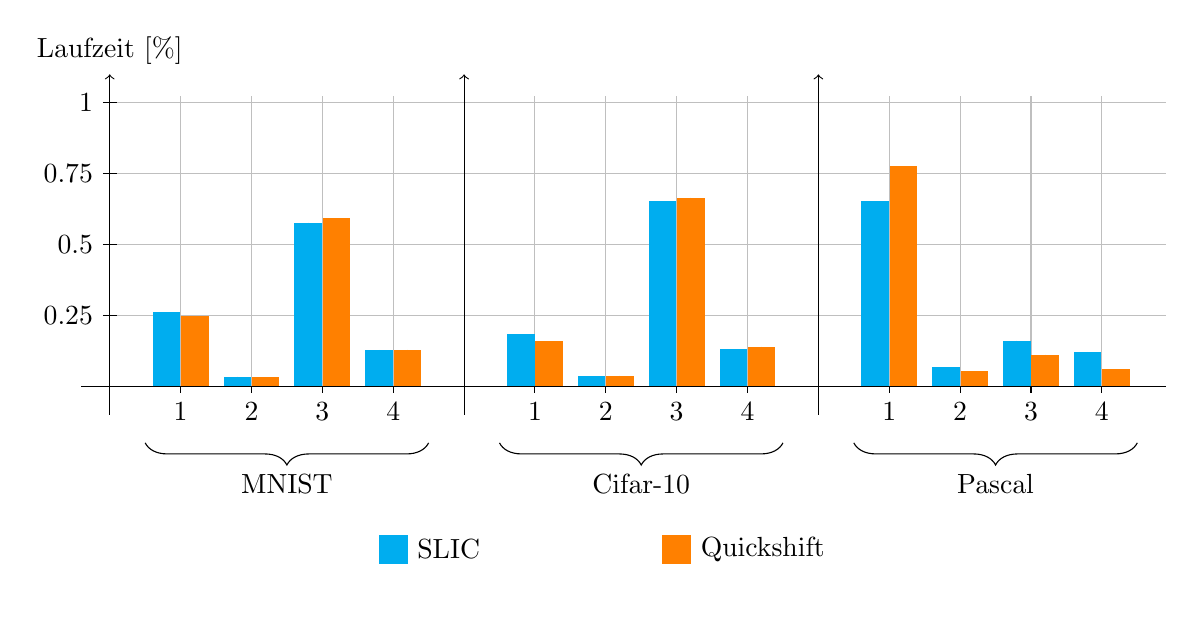
\begin{tikzpicture}[scale=0.9]
  \tikzstyle{slic}=[color=cyan, fill=cyan]
  \tikzstyle{quickshift}=[color=orange, fill=orange]

  \fill[white] (0, -2.9) rectangle (1, -1) node {};  % Abstand nach unten

  \draw[color=lightgray] (-0.1, -0.1) grid (14.9, 4.1);

  \draw[] (-0.4, 0) -- (14.9, 0);
  \draw[->] (0, -0.4) -- (0, 4.4) node[above] {Laufzeit [\%]};
  \draw[->] (5, -0.4) -- (5, 4.4);
  \draw[->] (10, -0.4) -- (10, 4.4);

  \draw (0.1, 1) -- (-0.1, 1) node[left] {$0.25$};
  \draw (0.1, 2) -- (-0.1, 2) node[left] {$0.5$};
  \draw (0.1, 3) -- (-0.1, 3) node[left] {$0.75$};
  \draw (0.1, 4) -- (-0.1, 4) node[left] {$1$};

  \draw[slic,       line width=0.35cm] (0.8, 0) -- (0.8, 1.0456);
  \draw[quickshift, line width=0.35cm] (1.2, 0) -- (1.2, 0.986);
  \draw (1, 0) -- (1, -0.1) node[below] {$1$};

  \draw[slic,       line width=0.35cm] (1.8, 0) -- (1.8, 0.1344);
  \draw[quickshift, line width=0.35cm] (2.2, 0) -- (2.2, 0.1224);
  \draw (2, 0) -- (2, -0.1) node[below] {$2$};

  \draw[slic,       line width=0.35cm] (2.8, 0) -- (2.8, 2.3084);
  \draw[quickshift, line width=0.35cm] (3.2, 0) -- (3.2, 2.3674);
  \draw (3, 0) -- (3, -0.1) node[below] {$3$};

  \draw[slic,       line width=0.35cm] (3.8, 0) -- (3.8, 0.5116);
  \draw[quickshift, line width=0.35cm] (4.2, 0) -- (4.2, 0.5148);
  \draw (4, 0) -- (4, -0.1) node[below] {$4$};

  \draw [decoration={brace,mirror,amplitude=8pt},decorate] (0.5,-0.8) -- node[below=8pt] {\gls{MNIST}} (4.5,-0.8);

  \draw[slic,       line width=0.35cm] (5.8, 0) -- (5.8, 0.7304);
  \draw[quickshift, line width=0.35cm] (6.2, 0) -- (6.2, 0.6336);
  \draw (6, 0) -- (6, -0.1) node[below] {$1$};

  \draw[slic,       line width=0.35cm] (6.8, 0) -- (6.8, 0.1388);
  \draw[quickshift, line width=0.35cm] (7.2, 0) -- (7.2, 0.1488);
  \draw (7, 0) -- (7, -0.1) node[below] {$2$};

  \draw[slic,       line width=0.35cm] (7.8, 0) -- (7.8, 2.61);
  \draw[quickshift, line width=0.35cm] (8.2, 0) -- (8.2, 2.6592);
  \draw (8, 0) -- (8, -0.1) node[below] {$3$};

  \draw[slic,       line width=0.35cm] (8.8, 0) -- (8.8, 0.5204);
  \draw[quickshift, line width=0.35cm] (9.2, 0) -- (9.2, 0.5584);
  \draw (9, 0) -- (9, -0.1) node[below] {$4$};

    \draw [decoration={brace,mirror,amplitude=8pt},decorate] (5.5,-0.8) -- node[below=8pt] {\gls{Cifar}-10} (9.5,-0.8);

  \draw[slic,       line width=0.35cm] (10.8, 0) -- (10.8, 2.6104);
  \draw[quickshift, line width=0.35cm] (11.2, 0) -- (11.2, 3.1044);
  \draw (11, 0) -- (11, -0.1) node[below] {$1$};

  \draw[slic,       line width=0.35cm] (11.8, 0) -- (11.8, 0.2636);
  \draw[quickshift, line width=0.35cm] (12.2, 0) -- (12.2, 0.2124);
  \draw (12, 0) -- (12, -0.1) node[below] {$2$};

  \draw[slic,       line width=0.35cm] (12.8, 0) -- (12.8, 0.6408);
  \draw[quickshift, line width=0.35cm] (13.2, 0) -- (13.2, 0.4432);
  \draw (13, 0) -- (13, -0.1) node[below] {$3$};

  \draw[slic,       line width=0.35cm] (13.8, 0) -- (13.8, 0.4852);
  \draw[quickshift, line width=0.35cm] (14.2, 0) -- (14.2, 0.24);
  \draw (14, 0) -- (14, -0.1) node[below] {$4$};

  \draw [decoration={brace,mirror,amplitude=8pt},decorate] (10.5,-0.8) -- node[below=8pt] {\gls{Pascal}} (14.5,-0.8);

  \tikzstyle{node}=[rectangle,draw, minimum width=10pt, minimum height=10pt, inner sep=0pt]
  \node[node, slic,       label=right:\gls{SLIC}] (1) at (4, -2.3) {};
  \node[node, quickshift, label=right:Quickshift] (2) at (8, -2.3) {};
\end{tikzpicture}

\begin{tabular}{ll}
  \toprule
  1. Segmentierung & 2. Adjazenzbestimmung\\
  3. Graphvergröberung (4 Ebenen) & 4. Merkmalsextraktion\\
  \bottomrule
\end{tabular}

\caption[Laufzeitverteilung der spektralen Vorverarbeitungsschritte]{Laufzeitverteilung der einzelnen Vorverarbeitungsschritte für das spektrale Lernen auf Graphen, unterteilt \bzgl{} unterschiedlichen Datensätze \gls{MNIST}, \gls{Cifar}-10 und \gls{Pascal} und den verwendeteten Superpixelalgorithmen \gls{SLIC} und Quickshift.
Wohingegen für \gls{MNIST} und \gls{Cifar}-10 die Graphvergröberung die längste Berechnungsdauer in Anspruch nimmt, zeigt sich dagegegen für größere Datensätze (\gls{Pascal}) die Segmentierung als Flaschenhals der Vorverarbeitung.}
\label{fig:laufzeit_spektral_pipeline}
\end{figure}


\paragraph{Vergleich \bzgl{} vorhandener Implementierungen}
\label{vergleich_laufzeit}

\begin{figure}[t]
\centering
  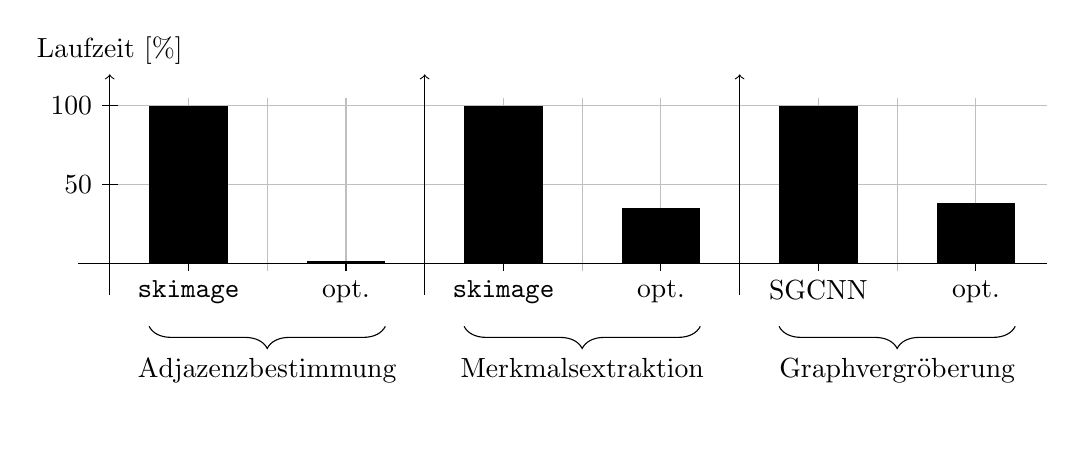
\begin{tikzpicture}[]
  \fill[white] (0, -2) rectangle (1, -1) node {};  % Abstand nach unten

  \draw[color=lightgray] (-0.1, -0.1) grid (11.9, 2.1);

  \draw[] (-0.4, 0) -- (11.9, 0);
  \draw[->] (0, -0.4) -- (0, 2.4) node[above] {Laufzeit [\%]};
  \draw[->] (4, -0.4) -- (4, 2.4);
  \draw[->] (8, -0.4) -- (8, 2.4);

  \draw (0.1, 1) -- (-0.1, 1) node[left] {$50$};
  \draw (0.1, 2) -- (-0.1, 2) node[left] {$100$};

  \draw[line width=1cm] (1, 0) -- (1, 2);
  \draw[line width=1cm] (3, 0) -- (3, 0.030153);
  \draw (1, 0) -- (1, -0.1) node[below] {\texttt{skimage}};
  \draw (3, 0) -- (3, -0.1) node[below] {opt.};
  \draw [decoration={brace,mirror,amplitude=8pt},decorate] (0.5,-0.8) -- node[below=8pt] {Adjazenzbestimmung} (3.5,-0.8);

  \draw[line width=1cm] (5, 0) -- (5, 2);
  \draw[line width=1cm] (7, 0) -- (7, 0.704036);
  \draw (5, 0) -- (5, -0.1)  node[below] {\texttt{skimage}};
  \draw (7, 0) -- (7,  -0.1) node[below] {opt.};
  \draw [decoration={brace,mirror,amplitude=8pt},decorate] (4.5,-0.8) -- node[below=8pt] {Merkmalsextraktion} (7.5,-0.8);

  \draw[line width=1cm] (9, 0)   -- (9, 2);
  \draw[line width=1cm] (11,  0) -- (11,  0.769867);
  \draw (9, 0)  -- (9, -0.1)  node[below] {\acs{SGCNN}};
  \draw (11, 0) -- (11, -0.1) node[below] {opt.};
  \draw [decoration={brace,mirror,amplitude=8pt},decorate] (8.5,-0.8) -- node[below=8pt] {Graphvergröberung} (11.5,-0.8);

\end{tikzpicture}

\begin{tabular}{lrrr}
  \toprule
  Vorverarbeitungsschritt & vorhanden [ms] & optimiert [ms] & Gewinn [\%]\\
  \midrule
  Adjazenzbestimmung & 866 & 13 & 6615\\
  Merkmalsextraktion & 144 & 50 & 288\\
  Graphvergröberung (4 Ebenen) & 87 & 33 & 264\\
  \bottomrule
\end{tabular}

\caption[Laufzeitvergleich \bzgl{} anderer Implementierungen]{Vergleich der Laufzeiten verschiedener Vorverarbeitungsschritte \bzgl{} des Lernens auf Graphen zwischen bereits vorhandenen, quelloffenen Implementierungen (links) und ihren jeweiligen entwickelten optimierten Versionen (rechts) am Beispiel eines Bildes aus \gls{Pascal}: (1) Adjazenzbestimmung einer Segmentierungsmaske, (2) Merkmalsextraktion und (3) Graphvergröberung inklusive der entsprechenden Anordung der Knoten zu binären Bäumen.
  In allen Bereichen konnten deutliche Laufzeitgewinne erreicht werden.}
\label{fig:laufzeit_vergleich}
\end{figure}

